\chapter{Implementation,Testing and Maintenance}
\section{Introduction to Languages, IDE's,Tools and Technologies Used For Implementation}
\subsection{Java}
Java is a very popular
programming language developed by Sun Microsystems (now owned by
Oracle). Developed long after C and C++, Java incorporates many of the
powerful features of those powerful languages while addressing some of
their drawbacks. Still, programming languages are only as powerful as
their libraries. These libraries exist to help developers build applications.\\
Some of the Java’s important core features are:\\
\begin{itemize}
\item It’s easy to learn and understand.
\item It’s designed to be platform-independent and secure, using virtual machines.
\item It’s object-oriented.
\end{itemize}
Android relies heavily on these Java fundamentals. The Android SDK
includes many standard Java libraries (data structure libraries, mathlibraries, graphics libraries, networking libraries and everything else you could want) as well as special Android libraries that will help you develop awesome Android applications.\\
\textbf{\emph{Platform Independence Importance}}\\
With many programming languages, you need to use a compiler to reduce
your code down into machine language that the device can understand.
While this is well and good, different devices use different machine
languages. This means that you might need to compile your applications
for each different device or machine language—in other words, your code
isn’t very portable. This is not the case with Java. The Java compilers
convert your code from human readable Java source files to something
called “bytecode” in the Java world. These are interpreted by a Java
Virtual Machine, which operates much like a physical CPU might operate
on machine code, to actually execute the compiled code. Although it might
seem like this is inefficient, much effort has been put into making this
process very fast and efficient. These efforts have paid off in that Java
performance in generally second only to C/C++ in common language
performance comparisons.\\
Android applications run in a special virtual machine called the Dalvik
VM. While the details of this VM are unimportant to the average
developer, it can be helpful to think of the Dalvik VM as a bubble in which
your Android application runs, allowing you to not have to worry about
whether the device is a Motorola Droid, an HTC Evo, or the latest toaster
running Android. You don’t care so long as the device is Dalvik VM
friendly—and that’s the device manufacturer’s job to implement, not
yours.\\
\textbf{\emph{Why is Java Secure?}}\\
Let’s take this bubble idea a bit further. Because Java applications run
within the bubble that is a virtual machine, they are isolated from the
underlying device hardware. Therefore, a virtual machine can encapsulate,
contain, and manage code execution in a safe manner compared to
languages that operate in machine code directly. The Android platform
takes things a step further. Each Android application runs on the (Linux-
based) operating system using a different user account and in its own
instance of the Dalvik VM. Android applications are closely monitored by
the s.operating system and shut down if they don’t play nice (e.g. use toomuch processing power, become unresponsive, waste resources, etc.).\\
Therefore, it’s important to develop applications that are stable and
responsive. Applications can communicate with one another using well-
defined protocol.


\subsection{Android Development Tools}
\begin{itemize}
\item \textbf{\emph{Android SDK:}}\\
The Android Software Development Kit (Android SDK) contains the
necessary tools to create, compile and package Android applications. Most
of these tools are command line based. The primary way to develop
Android applications is based on the Java programming language.
\item \textbf{\emph{Android debug bridge (adb):}}\\
The Android SDK contains the Android debug bridge (adb), which is a
tool that allows you to connect to a virtual or real Android device, for the
purpose of managing the device or debugging your application.
\item \textbf{\emph{Android Developer Tools and Android Studio:}}\\
Google provides two integrated development environments (IDEs) to
develop new applications.The Android Developer Tools (ADT) are based on the Eclipse IDE. ADT
is a set of components (plug-ins), which extend the Eclipse IDE with
Android development capabilities.
Google also supports an IDE called Android Studio for creating Android
applications. This IDE is based on the IntelliJ IDE.\\
Both IDEs contain all required functionality to create, compile, debug and
deploy Android applications. They also allow the developer to create and
start virtual Android devices for testing.\\
Both tools provide specialized editors for Android specific files. Most of
Android's configuration files are based on XML. In this case these editors
allow you to switch between the XML representation of the file and a
structured user interface for entering the data.Dalvik Virtual Machine
The Android system uses a special virtual machine, i.e., the Dalvik Virtual
Machine (Dalvik) to run Java based applications. Dalvik uses a custom
bytecode format which is different from Java bytecode.
\\
Therefore you cannot run Java class files on Android directly; they need to
be converted into the Dalvik bytecode format.
\item \textbf{\emph{Android RunTime (ART):}}\\
With Android 4.4, Google introduced the Android RunTime (ART) as
optional runtime for Android 4.4. It is expected that versions after 4.4 will
use ART as default runtime. ART uses Ahead Of Time compilation. During the deployment process of
an application on an Android device, the application code is translated into
machine code. This results in approx. 30\% larger compile code, but allows
faster execution from the beginning of the application.

\end{itemize}

\subsection{Security and Permission Concept in Android}

\begin{itemize}
\item \textbf{\emph{Security Concept In Android:}}\\
The Android system installs every Android application with a unique user
and group ID. Each application file is private to this generated user, e.g.,
other applications cannot access these files. In addition each Android
application is started in its own process.\\

Therefore, by means of the underlying Linux kernel, every Android
application is isolated from other running applications.
If data should be shared, the application must do this explicitly via an
Android component which handles the sharing of the data, e.g., via a
service or a content provider.

\item \textbf{\emph{Permission concept in Android:}}\\
Android contains a permission system and predefines permissions for
certain tasks. Every application can request required permissions and also
define new permissions. For example, an application may declare that it
requires access to the Internet.\\

Permissions have different levels. Some permissions are automatically
granted by the Android system, some are automatically rejected. In most
cases the requested permissions are presented to the user before installing
the application. The user needs to decide if these permissions shall be
given to the application.\\

If the user denies a required permission, the related application cannot be
installed. The check of the permission is only performed during
installation, permissions cannot be denied or granted after the installation.\\

An Android application declares the required permissions in itsAndroidManifest.xml configuration file. It can also define additional
permissions which it can use to restrict access to certain components.
\end{itemize}


%%%%%%%%%%%%%%%%%%%%%%%%%%%%%%%%%%%%%%%%%%%%%%

\pagebreak
\section{Coding Standards of Language Used}
Coding Standards of Java are used in the whole project. This standard include the following:
\begin{itemize}
\item No wildcard imports.
\item Overloads appear sequentially.
\item Braces are used even when the body is empty or contains a single statement.
\item Two space indentation.
\item Column limit can be 80 or 100 characters.
\item No C-style array declarations.
\item Default statements required in switch statements.
\item Modifiers appear in the order recommended by the Java Language Specification.
\item Constants use CONSTANT\_CASE. Note that every constant is a static final field, but not all static final fields are constants.
\item Class name should start with uppercase letter.
\item Function name should start with lowercase letter.
\end{itemize}
%%%%%%%%%%%%%%%%%%%%%%%%%%%%%%%%%%%%%%%%%%%%%%%%%%%%
\pagebreak
\section{Project Scheduling}
Project scheduling is concerned with the techniques that can be employed to manage the activities that need to be undertaken during the development of a project. Scheduling is carried out in advance of the project commencing and involves:
\begin{itemize}
\item Identifying the tasks that need to be carried out.
\item Estimating how long they will take.
\item Allocating resources (mainly personnel).
\item Scheduling when the tasks will occur.
\end{itemize}
Once the project is underway control needs to be exerted to ensure that the plan continues to represent the best prediction of what will occur in the future based on what occurs during the development and often necessitates revision of the plan.
Effective project planning will help to ensure that the systems are delivered:
\begin{itemize}
\item Within cost;
\item Within the time constraint;
\item To a specific standard of quality.
\end{itemize}

Two project scheduling techniques will be presented, the Milestone Chart and Gantt Chart.
\begin{enumerate}
\item \textbf{\emph{Milestone Charts:}}\\
Milestones mark significant events in the life of a project, usually critical activities which must be achieved on time to avoid delay in the project. Milestones should be truely significant and be reasonable in terms of deadlines (avoid using intermediate stages).
\\
Examples include:
\begin{itemize}
\item Installation of equipment.
\item Completion of phases.
\item File conversion.
\item Cut over to the new system
\end{itemize}

\item \textbf{\emph{Gantt Charts:}}\\
A Gantt chart is a horizontal bar or line chart which will commonly include the following features:
\begin{itemize}
\item Activities identified on the left hand side.
\item Time scale is drawn on the top (or bottom) of the chart.
\item A horizontal open oblong or a line is drawn against each activity indicating estimated duration.
\item Dependencies between activities are shown.
\item At a review point the oblongs are shaded to represent the actual time spent (an alternative is to represent actual and estimated by 2 separate lines).
\item A vertical cursor (such as a transparent ruler) placed at the review point makes it possible to establish activities which are behind or ahead of schedule.
\end{itemize}
\end{enumerate}

Following is the chart of various commits on github, while developing this application:
\begin{figure}[H]
\centering 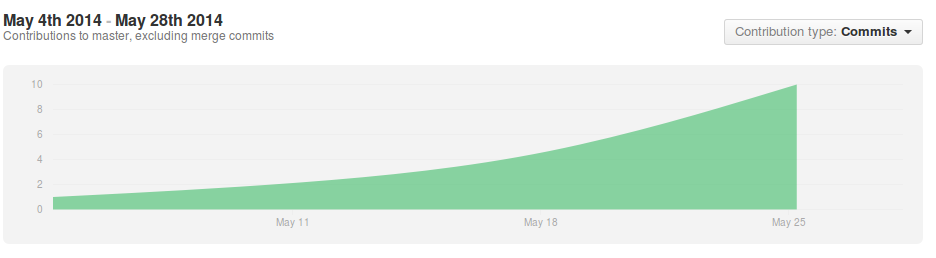
\includegraphics[scale=0.4]{image/commit.png}
\caption{Graph of Commits on GitHub}
\end{figure}
This graph is showing commit in last week of May. It depicts how many times, changes are pushed on to githu after testing.
\begin{figure}[H]
\centering 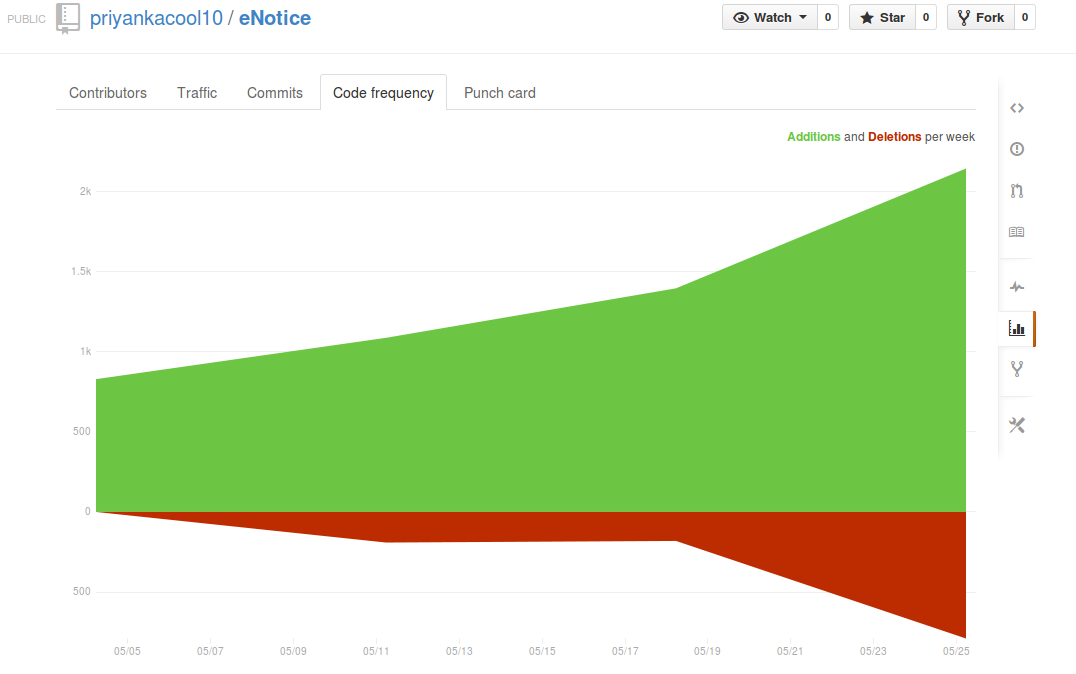
\includegraphics[scale=0.4]{image/codefrequency.png}
\caption{Code Frequency Graph on GitHub}
\end{figure}
This graph depicts the frequency of code that is pushed on github on respective dates.

%%%%%%%%%%%%%%%%%%%%%%%%%%%%%%%%%%%%%%%%%%%%%%%%%%%%%%%%%%%
\pagebreak
\section{Test Plan and Test Activities}
\subsection{Test Plan}
A test plan can be defined as a document describing the scope, approach, resources, and schedule of intended testing activities. It identifies test items, the features to be tested, the testing tasks, who will do each task, and any risks requiring contingency planning.
In software testing, a test plan gives detailed testing information regarding an upcoming testing effort, including\\
\begin{itemize}
\item Scope of testing
\item Schedule
\item Test Deliverables
\item Release Criteria
\item Risks and Contingencies 
\end{itemize}
It is also be described as a detail of how the testing will proceed, who will do the testing, what will be tested, in how much time the test will take place, and to what quality level the test will be performed.\\

The process of defining a test project so that it can be properly measured and controlled. The test planning process generates a high level test plan document that identifies the software items to be tested, the degree of tester independence, the test environment, the test case design and test measurement techniques to be used, and the rationale for their choice.\\

A testing plan is a methodological and systematic approach to testing a system such as a machine or software. It can be effective in finding errors and flaws in a system. In order to find relevant results, the plan typically contains experiments with a range of operations and values, including an understanding of what the eventual workflow will be.\\

Test plan is a document which includes, introduction, assumptions, list of test cases, list of features to be tested, approach, deliverables, resources, risks and scheduling. A test plan is a systematic approach to testing a system such as a machine or software. The plan typically contains a detailed understanding of what the eventual workflow will be.
A record of the test planning process detailing the degree of tester indedendence, the test environment, the test case design techniques and test measurement techniques to be used, and the rationale for their choice.

\subsection{Test Activities}
Various Testing Activities are as follow:
\begin{enumerate}
\item \textbf{\emph{Black box testing –}} Internal system design is not considered in this type of testing. Tests are based on requirements and functionality.

\item \textbf{\emph{White box testing –}} This testing is based on knowledge of the internal logic of an application’s code. Also known as Glass box Testing. Internal software and code working should be known for this type of testing. Tests are based on coverage of code statements, branches, paths, conditions.

\item \textbf{\emph{Unit testing –}} Testing of individual software components or modules. Typically done by the programmer and not by testers, as it requires detailed knowledge of the internal program design and code. may require developing test driver modules or test harnesses.

\item \textbf{\emph{Incremental integration testing –}} Bottom up approach for testing i.e continuous testing of an application as new functionality is added; Application functionality and modules should be independent enough to test separately. done by programmers or by testers.

\item \textbf{\emph{Integration testing –}} Testing of integrated modules to verify combined functionality after integration. Modules are typically code modules, individual applications, client and server applications on a network, etc. This type of testing is especially relevant to client/server and distributed systems.

\item \textbf{\emph{Functional testing –}} This type of testing ignores the internal parts and focus on the output is as per requirement or not. Black-box type testing geared to functional requirements of an application.

\item \textbf{\emph{System testing –}} Entire system is tested as per the requirements. Black-box type testing that is based on overall requirements specifications, covers all combined parts of a system.

\item \textbf{\emph{End-to-end testing –}} Similar to system testing, involves testing of a complete application environment in a situation that mimics real-world use, such as interacting with a database, using network communications, or interacting with other hardware, applications, or systems if appropriate.

\item \textbf{\emph{Acceptance testing -}} Normally this type of testing is done to verify if system meets the customer specified requirements. User or customer do this testing to determine whether to accept application.

\item \textbf{\emph{Usability testing –}} User-friendliness check. Application flow is tested, Can new user understand the application easily, Proper help documented whenever user stuck at any point. Basically system navigation is checked in this testing.
\end{enumerate}
